
\begin{figure}[h]
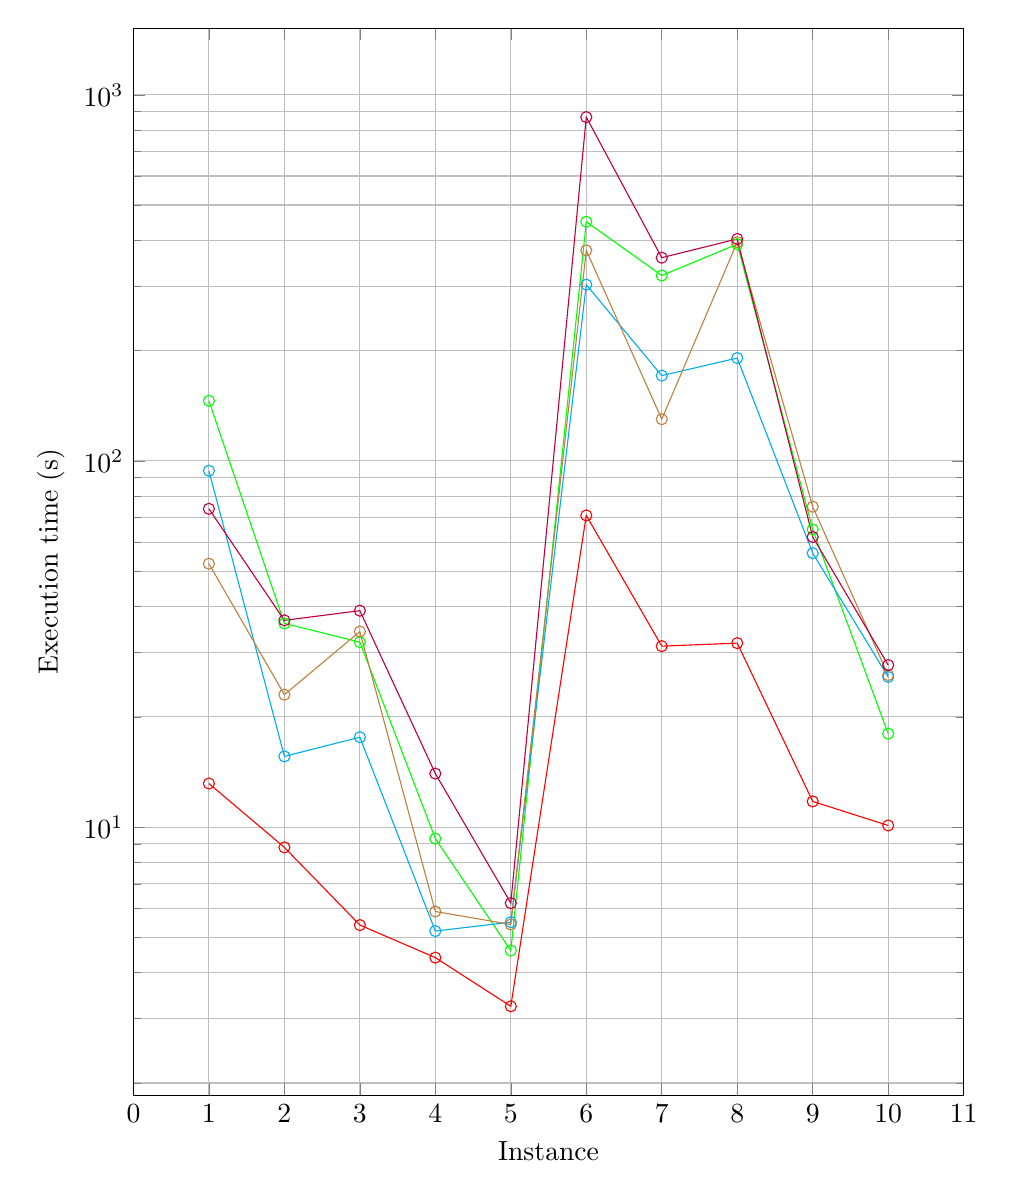
\begin{tikzpicture}
	\begin{axis}[width=\textwidth,height=100ex,
		xlabel=Instance,
		ylabel=Execution time (s), xmin=0, ymin=0, grid=both,
		ymode=log]

% gurobi p1
\addplot[mark=o,color=red] coordinates {
(1, 13.152454848)
(2, 8.8)
(3, 5.4)
(4, 4.4)
(5, 3.24)
(6, 70.99)
(7, 31.2)
(8, 31.8)
(9, 11.75)
(10, 10.1)
};

% cbc nothing
\addplot[mark=o,color=green] coordinates {
(1, 146)
(2, 36)
(3, 32)
(4, 9.3)
(5, 4.6)
(6, 450.1)
(7, 321)
(8, 391)
(9, 65)
(10, 18)
};

% cbc with random heuristic
\addplot[mark=o,color=cyan] coordinates {
(1, 94)
(2, 15.6)
(3, 17.6)
(4, 5.2)
(5, 5.5)
(6, 303)
(7, 171)
(8, 191)
(9, 56)
(10, 25.7)
};

% cbc with ff heuristic
\addplot[mark=o,color=brown] coordinates {
(1, 52.4)
(2, 23)
(3, 34.2)
(4, 5.88)
(5, 5.42)
(6, 376)
(7, 130)
(8, 396)
(9, 75)
(10, 26)
};

% cbc with divisor 100
\addplot[mark=o,color=purple] coordinates {
(1, 74)
(2, 36.7)
(3, 39)
(4, 14)
(5, 6.2)
(6, 869)
(7, 359)
(8, 404)
(9, 62)
(10, 27.7)
};

\end{axis}

\end{tikzpicture}%
\caption{Execution time for all relevant cases using P1. Red: Gurobi, green: Cbc without any optimization, cyan: Cbc using the random heuristic, brown: Cbc using the farthest-first heuristic, purple: Cbc using the VI attempt with divisor 100.}
\end{figure}
